% Tento soubor nahraďte vlastním souborem s obsahem práce.
%=========================================================================
% Autoři: Michal Bidlo, Bohuslav Křena, Jaroslav Dytrych, Petr Veigend a Adam Herout 2019

% Pro kompilaci po částech (viz projekt.tex), nutno odkomentovat a upravit
%\documentclass[../projekt.tex]{subfiles}
%\begin{document}

\newtheorem{definition}{\textbf{Definice}}

\chapter{Úvod}
\label{uvod}

Umělá inteligence je obor, který nás postupem let všechny obkopuje čím dál tím více.
Dokonce je navždy spjata i s naším českým národem, když Karel Čapek dal zrodu slova robot.

Pokrok umělé inteligence je často měřen aplikací v oblasti her.
Hry jsou vhodným ukazatelem pokroku v oblasti umělé inteligence, protože mají jasná pravidla, výkon je snadno měřitelný a pokrok dokáže vidět i lajk.
Umělá inteligence již dokázala porazit nejlepší hráče v šachu \cite{DeepBlue}, Dota 2 \cite{Dota2} a Go \cite{AlphaGo}.

Hra studovaná v této práci je hra Scotland Yard.
Je to hra pro tři až šest hráčů.
V této hře obvykle hraje jeden hráč jako Pan X, který se snaží uniknout policistům, ovládanými ostatními hráči.
Policisté avšak nevědí, kde na herním poli se Pan X nachází.
Musí tedy odhadovat jeho pozici a spolupracovat mezi sebou, aby ho mohli polapit.
Pozice Pana X je odhalena pouze v určitých kolech.
Hra končí, když je Pan X chycen (vyhrávají policisté), nebo když je dosažen maximální počet kol (vyhrává Pan X).
Scotland Yard je ideální hrou pro studování umělé inteligence, protože je hra s neúplnou informací a k vítězství policistů je zapotřebí spolupráce.

Zaměření této práce jsem si vybral jelikož mi vždy byla umělá inteligence blízká a vždy jsem chtěl .
Avšak jsem nikdy nenašel odhodlání ponořit se do této oblasti.

Rozhodl jsem se pro bližší zkoumání algoritmů posilovaného učení, konkrétně algoritmu PPO (Proximal Policy Optimization).
Tento algoritmus je často používán pro řešení problémů se spojitými veličinamy a ve 3D prostoru.
Dle provedených studií je vhodný pro řešení problémů s neúplnou informací \cite{Manille} a je vhodný pro hry na schování a hledání \cite{PPO_Hide_Seek}.
Proto je pro mě zajímavý a zkušenost s tímto algoritmém by se dala využít v mém pracovním životě.

Pro zpracování práce byl využity tyto hlavní knihovny:
\begin{itemize}
  \item \emph{Ray.Rlib} - knihovna s implementací algoritmu PPO
  \item \emph{PyTorch} - podpůrná knihovna Ray.Rlib
  \item \emph{TensorFlow} - podpůrná knihovna Ray.Rlib
  \item \emph{Gym} - knihovna pro vytvoření prostředí pro učení
  \item \emph{Pygame} - knihovna pro vytváření uživatelského rozhraní
\end{itemize}


\chapter{Shrnutí dosavadního stavu}
\label{dosavadni-stav}

\begin{itemize}
  \item \emph {40-50\,\% rozsahu práce}
  \item \emph{Hodně citovat literaturu}
  \item \emph{Vysvětlit všechno, už ne pro plebíky}
  \item \emph{Je vhodné na začátku této části uvést, co obsahuje a proč a taky že „není encyklopedickým přehledem“}
  \item \emph{Asi tak ze 2 kapitol?}
  \item \emph{Existující řešení (implementace scotlandu, říct že se implementuje pomocí tamtoho algoritmu a proč jsem vzal PPO)}
\end{itemize}


\section{Desková hra Scotland Yard}

Scotland Yard je populární hra pro tři a více hráčů, která kombinuje prvky schovávané a hry na honěnou.
Jeden hráč hraje za Pana X, který se snaží uniknout policistům, ovládanými ostatními hráči.
Hra končí, když je Pan X chycen (vyhrávají policisté), nebo když je dosažen maximální počet kol (vyhrává Pan X).
Originální hra se odehrává v Londýně.
Na herní mapě se nachází 200 polí, které jsou vzájemně propojené náhodnými cestami.
Každá cesta povoluje určitý způsob pohybu (např.
pouze taxíkem, pouze autobusem, atd.).
Jednotliví hráči využívají prvky veřejné dopravy k pohybu po herní ploše, kterými jsou:
\begin{itemize}
  \item \emph{Taxi}
  \item \emph{Autobus}
  \item \emph{Metro}
  \item \emph{Trajekt}
\end{itemize}

\begin{figure}[hbt]
	\centering
	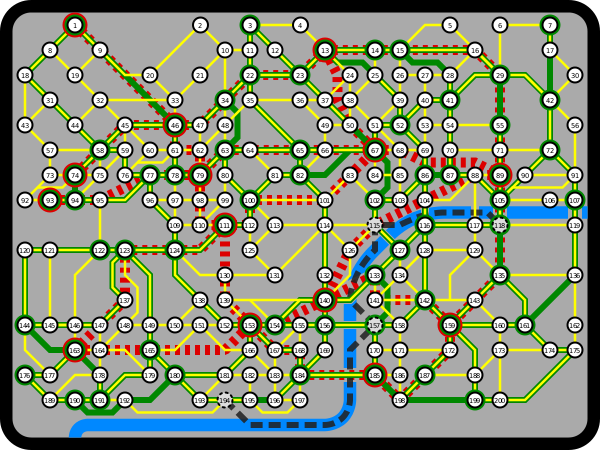
\includegraphics[width=0.9\textwidth]{obrazky-figures/scotland_original.png}
	\caption{Ukázka herní mapy pro hru Scotland Yard.
  Zdroj:\cite{scotland_original_image}}
\end{figure}

Každému hráči je na začátku hry přidělen pouze určitý počet jízdenek na tyto dopravní prostředky.
Pro využití dopravy je potřebná právě tato jízdenka.
Pokud ji hráč nemá, nemůže již tento způsob přepravy použít.
Hra se dělí na kola, ve kterých se hráči střídají.

Hlavní myšlenkou hry je, že po většinu kol je pozice Pana X je policistům utajena.
Odhaluje se jim pouze určená kola.
To znamená, že policisté musí odhadovat další kroky Pana X aby ho mohli polapit.
Tímto se ze hry Scotland Yard stává hra s neúplnou informací, jelikož policisté nevidí přesnou pozici Pana X.
Tento fakt ji činí vhodnou pro studování a rozvíjení oboru umělé inteligence.

\section{Bayesovské hry: Hry s neúplnou informací}
V oblasti umělé inteligence hraje důležitou roli modelování a řešení her.
Hry představují abstraktní formalizaci konfliktních interakcí mezi aktéry, tzv.
hráči.
Klasická teorie her se zaměřuje na hry s úplnou informací, kde mají všechny strany v daném okamžiku přístup ke všem relevantním informacím z herního prostředí.
V praxi se však častěji setkáváme se situacemi kde jednotlivým stranám chybí určité informace.
Tyto případy lze modelovat pomocí her s neúplnou informací, kde hráči nemají úplné znalosti o prostředí či soupeřích.
Neúplnou informaci můžeme sledovat například v:
\begin{itemize}
  \item \emph{Ekonomii} - kde se jedná o neúplnou informaci o trhu, cenách, situačních výkyvech, atd.
  \item \emph{Vojenské strategii} - kde se jedná o neúplnou informaci o pozici nepřítele, jeho vybavení, strategii, cíli, atd.
  \item \emph{Sportovní hry} - kde se jedná o neúplnou informaci o taktice soupeře, jeho schopnostech, atd.
\end{itemize}

\begin{definition}[Bayesovská hra]
\cite{Y_Narahari} je definována pěticí $(N, A_i, \theta_i, p(\theta_i), u_i)$, kde:

\begin{itemize}
\item $N$ je konečná množina hráčů, $N = \{1, 2, \ldots, n\}$.
\item $A_i$ je neprázdná množina strategií hráče $i$.
\item $\theta_i$ je neprázdná množina typů hráče $i$.
\item $p(\theta_i)$ je apriorní pravděpodobnostní rozdělení typu hráče $i$ na $\theta_i$.
\item $u_i: A_1 \times \cdots \times A_n \times \theta_1 \times \cdots \times \theta_n \rightarrow \mathbb{R}$ je výplatní funkce hráče $i$.
\end{itemize}
\end{definition}
Bayesovské hry představují formální rámec pro modelování her s neúplnou informací.

\subsection*{Stratego}

Stratego je desková strategická hra pro dva hráče, která se odehrává na hracím plánu rozděleném do políček a využívá se k ní sada figurek reprezentujících armádu.
Vychází z dřívějších her, jako je Šachy a Go, a kombinuje strategické plánování, taktické manévry.

Cílem hry je porazit soupeře nalezením a obsazením jeho vlajky.
Hráči to dělají tak, že se navzájem utkávají se svými figurkami na herním plánu.

Každý hráč má 40 figur, rozdělených do 11 hodností (generál, plukovník, skaut, atd.).
Figury lze rozeznat jen z jedné strany, proto oponent neví o jakou figuru se jedná.
Hráči se střídají v tazích, kdy se snaží najít oponentovu vlajku.
Hra začíná tím, že každý hráč rozmístí své figury na herní pole.
Hráči se střídají v tazích, kdy se snaží najít oponentovu vlajku.
Pokud hráč táhne na pole, kde se nachází oponentova figura, nastává souboj.
Souboj spočívá v odkrytí obou figur a vyhrává ta s vyšší hodností.
Figura, která vyhrála zůstává, poražená figura je odstraněna z hry.
Ve hře Stratego je důležité blafování a odhadování soupeřových tahů.

\begin{figure}[hbt]
	\centering
	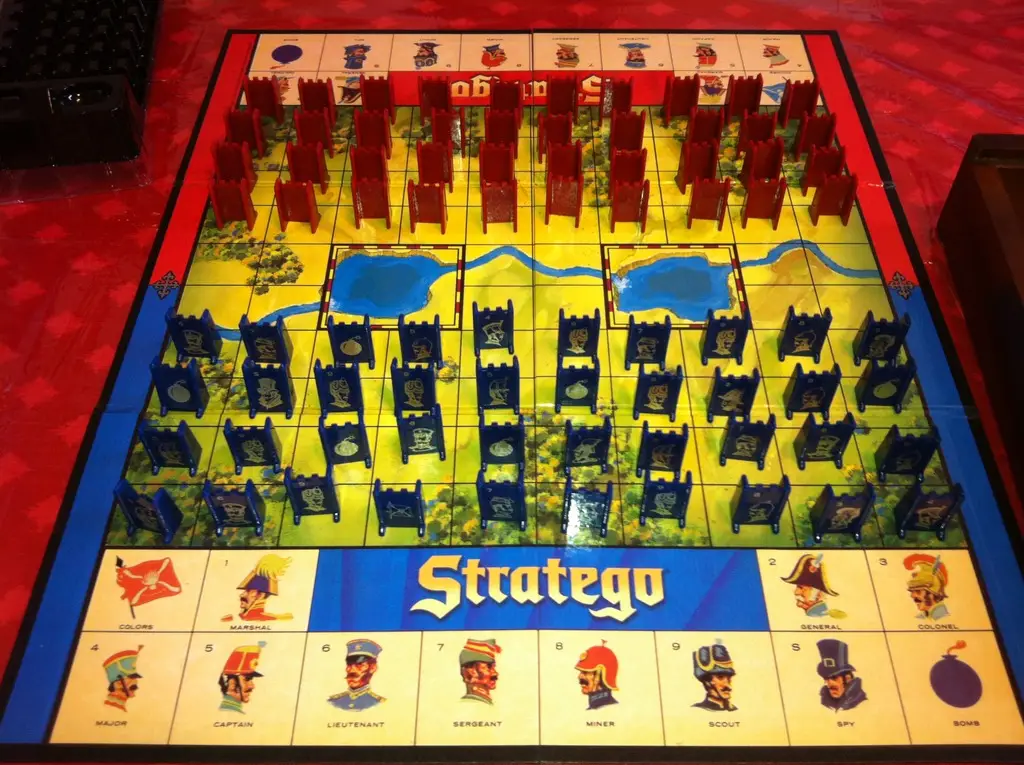
\includegraphics[width=0.6\textwidth]{obrazky-figures/stratego.png}
	\caption{Ukázka rozestavěných figur ve hře Stratego.
  Zdroj:\cite{Stratego_image}}
\end{figure}

Z pohledu umělé inteligence je Stratego zapeklitý problém.
Nejenže je hra s neúplnou informací a je tedy zapotřebí odhadovat oponentovy tahy a blafovat, ale také je hra s velkým prostorem stavů $10^{535}$\cite{Perolat_2022}.
Až do roku 2022 se AI nepodařilo porazit expertního hráče v této hře.
To se změnilo příchodem \emph{DeepNash}\cite{Perolat_2022}, kdy se tato metoda umístila mezi 3 nejlepšími hráči světa.


\section{Klíčové koncepty posilovaného učení}
Posilované učení (Reinforcement Learning, RL) je oblast strojového učení, která se zaměřuje na učení agentů v dynamickém prostředí.
Agent se učí strategii chování, která maximalizuje kumulativní odměnu.

\subsection{Agent}

Je komplexní entita, která interaguje s prostředím.
Prostředí poskytuje agentovi informace o stavu a agent na základě těchto pozorování vykonává akce.
Tyto akce mohou ovlivnit stav prostředí a agent obdrží odměnu na základě odměnové funkce.
Agent volí takové akce aby maximalizoval kumulativní odměnu.

\subsection{Prostředí}

Je vše s čím agent interaguje.
Prostředí je buď fyzické (entity z reálného světa, ovládání chytré domácnosti, ovládání reaktoru, atd.) nebo virtuální (simulace, například hra).
Prostředí reaguje na akce agenta poskytuje mu zpětnou vazbu ve formě odměny či trestu (záporná odměna).
Pokud v prostředí existuje více agentů, může mít každý agent jiné pozorování.
Diky tomuto můžeme například schovat agentu \textit{A} určité informace, které agent \textit{B} vidí.

\subsection{Model}

Je matematická funkce, která popisuje chování prostředí v závislosti na agentových akcích.
Model může být známý nebo neznámý, to následně rozděluje metody učení posilovaného na 2 základní kategorie: metody \emph{s modelem} a metody \emph{ bez modelu}.


\subsection{Politika}

Pomocí posilovaného učení vzniká takzvaná politika.
Politika je matematická funkce, která definuje agentovo chování na základě jeho pozorování (stavu).
Snaží se definovat takové chování, které vede k maximální kumulativní odměně.
Politika může být deterministická nebo stochastická.


  \subsubsection{Deterministická politika}
  
  Deterministická politika přesně definuje cílový stav přechodu pro každý stav.
  Agent tedy pro jeden stav vždy volí stejnou akci.
  Tato politika je vhodná pokud je zapotřebí v každém stavu reagovat konzistentně, bez odchylek.
  Například, pokud agent ovládá termostat v domě a teplota je pod požadovanou hladinu.
  Nemůže se stát aby byla šance, že agent zvolí akci, která teplotu ještě sníží.
  Další výhoda, je že je jednoduchá na interpretaci a implementaci.\cite{Policies}

  \subsubsection{Stochastická politika}
  
  Zato stochastická politika definuje pro každý stav pravděpodobnostní rozdělení nad množinou akcí.
  Výsledná akce je tedy náhodná dle rozdělení pravděpodobnosti.
  Může tedy nastat situace kdy pro jeden stav agent zvolí jinou akci.
  Tato politika je vhodná pro situace, kdy je potřeba zkoumat různé strategie a kdy agent nemá úplnou informaci o prostředí.
  Například tam kde by deterministická politika zvolila jasnou akci \textit{A}, stochastická politika by mohla  s malou pravděpodobností zvolit akci \textit{B}.
  Čímž ale může odhalit, že stav \textit{B} je s ohledem na komulativní odměnu lepší než stav \textit{A}.\cite{Policies}


  \subsection{Akce}

  Akce je přechod z aktuálního stavu, do následujícího stavu z množiny možných stavů.
  Zjednodušeně, je to rozhodnutí, které agent vykonává v prostředí a toto rozhodnutí ovlivňuje prostředí.
  Akce zvolena dle politiky a je závislá na pozorování agenta.
  
  \subsection{Odměna}

  Odměna je hodnota, kterou agent obdrží od prostředí po vykonání akce.
  Může být kladná, záporná nebo nulová.
  Dle této zpětné vazby se agent učí, jak moc byla jeho zvolená akce v daném stavu vhodná.

\subsection{Hodnotová funkce}

  Hodnotová funkce vyhodnocuje, jak dobrý je stav tím, že predikuje budoucí odměnu.
  Čím vzdálenější odměna je, tím více je snížena.
  Jelikož, čím je odměna vzdálenější tím více je nejistá.

  Existují dva typy hodnotových funkcí:

  \subsubsection{Hodnotová funkce stavu $V(s)$}

  Hodnotová funkce stavu \emph{$V(s)$} vyhodnocuje očekávanou komulativní odměnu, pokud se agent nachází v tomto stavu.
  Tato funkce je závislá na politice, kterou se agent řídí.
  Vyhodnocuje tedy jak příznivý je daný stav pro agenta.

  \subsubsection*{Hodnotová funkce akce $Q(s, a)$}

  Hodnotová funkce akce \emph{$Q(s, a)$} vyhodnocuje očekávanou komulativní odměnu, pokud se agent nachází v tomto stavu a zvolí tuto akci.
  Tato funkce je opět závislá na politice, kterou se agent řídí.
  Vyhodnocuije tedy jak příznié je zvolení dané akce v aktuálním stavu.


\subsection{Markovský rozhodovací proces}

Teměř všechny problémy, řešené posilovaným učením, mohou být označeny jako Markovy rozhodovací procesy (Markov Decision Process).
Tato abstrakce je základním kamenem pro modelování algoritmů posilovaného učení.
Markovský rozhodovací proces značí, že následující stav není závislý na stavech minulých, nýbrž pouze na aktuálním stavu.

\begin{figure}[hbt]
	\centering
	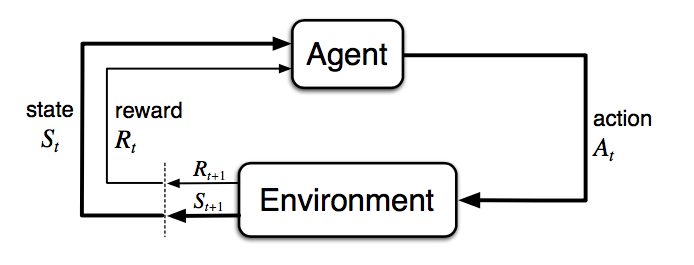
\includegraphics[width=0.6\textwidth]{obrazky-figures/RL_basics.png}
	\caption{Interakce mezi prostředím a agentem podle Markova rozhodovacího procesu.
  Zdroj:\cite{RL_basics}}
\end{figure}

\begin{definition}
  
Markovský rozhodovací proces je definován pěticí $(S, A, P, R, \gamma)$\cite{RL_basics}, kde:

\begin{itemize}
\item $S$ je množina stavů.

\item $A$ je množina akcí.
\item $P$ je pravděpodobnostní přechodová funkce
\item $R$ je odměnová funkce
\item $\gamma$ je diskontní faktor pro budoucí odměny
\end{itemize}
\end{definition}
\subsection{Bellmanova rovnice}

Belmanova rovnice se zamuřuje na rozložení hodnotových funkcí na menží snadněji zpracovatelné celky.
Dociluje toho tak, že rozděluje hodnotovou funkci na dvě části: \emph{okamžitou odměnu} a postupně snižovanou \emph{budoucí odměnu}.

\begin{equation}
  V(s) = E[R_{t+1} + \gamma V(S_{t+1}) | S_t = s]
\end{equation}

\begin{equation}
  Q(s, a) = E[R_{t+1} + \gamma E_{a\sim\pi}Q(S_{t+1}, a) | S_t = s, A_t = a]
\end{equation}

\subsection{Rovnováha mezi explorací a exploatací (exploration-exploitation)}



\subsection*{Rozdíl mezi nekompletní a neúplnou informací}


\section{Vhodné algoritmy pro řešení her s neúplnou informací}

Tato kapitola se zaměřuje na algoritmy, které jsou vhodné pro řešení her s neúplnou informací, s důrazem na metody posilovaného učení a srovnáním s klasickými metodami jako Monte Carlo.

\subsection*{Monte Carlo}
Metoda Monte Carlo (MC) je pravděpodobnostní metoda, která využívá simulaci hry anásledné odhady hodnoty stavu.

\subsection*{Q-learning}
\subsection*{Deep Q-learning}
\subsection*{Metody gradientu politiky}
\subsubsection*{Věta o gradientu politiky}
\section{Proximální optimalizace politiky}
\label{sec:proximalni-optimalizace-politiky}

\section{Algoritmus PPO}

\chapter{Zhodnocení současného stavu a plán práce (návrh)}
\label{navrh}
\begin{itemize}
  \item \emph {Kritické zhodnocení dosavadního stavu}
  \item \emph {Návrh, co by bylo vhodné vyřešit na základě znalostí dosavadního stavu}
  \item \emph {Co jste konkrétně udělal s teorií popsanou výše}
  \item \emph {Volba OS, jazyk, knihovny}
  \item \emph {Detailní rozbor zadání práce, detailní specifikace a formulace cíle a jeho částí}
  \item \emph {Popis použití řešení, situace/problémy, které projekt řeší}
  \item \emph {Postup práce/kroky vedoucí k cíli, rozdělení celku na podčásti}
  \item \emph {Návrh celého řešení i jeho částí, s odkazy na teoretickou část}
\end{itemize}

\section*{Zkoumaná modifikovaná verze hry Scotland Yard}

Tato práce využívá modifikovanou verzi hry Scotland Yard, ve které se hráči pohybují po mřížkové herní ploše ve tvaru čtverce.
Na mřížce se nachází {\color{red}[15x15]} polí.
Hračí se po těchto polích pohybují ortogonálně i diagonálně, vždy o maximálně 1 pole.
Hráč se může rozhodnot nezměnit pozici a zůstat na svém aktuálním poli.
K pohybu nejsou potřebné žádné jízdenky.
Toto zjednodušení herní plochy nijak nemění základní podstatu hry, zachovává neurčitost, ale značně zjednodušuje implementaci.
Hra začíná tím, že se vyberou náhodné možné pozice Pana X a policistů.
Z těchto možných pozíc se následně náhodná pozice přidělí jednotlivým hráčům.



\section*{Implementace umělé inteligence do hry Scotland Yard pomocí algoritmu PPO}
\label{implementace}

\subsection*{Vizuální stránka}

\subsection*{Prostředí}

\subsection*{Učení}

//zmínit, že ray rlib neumí action mapping, takže nejde zamezit zvolení jistých akcí.
Proto jsou možné i nevalidní akce. Ale jsou velmi penalizovány.

\chapter{Experimenty}
\label{experimenty}
\chapter{Závěr}
\label{zaver}
\chapter{Přílohy}
\label{prilohy}



%===============================================================================

% Pro kompilaci po částech (viz projekt.tex) nutno odkomentovat
%\end{document}
